\subsection{RunMultiStream}

\subsubsection*{Results}

\textbf{Test 1}

Event sources = 2

EventSource.minTimes = [ 10, 20, 30, 40, 50, 10, 20, 30, 40 ]

EventSource.maxTimes = [ 100, 150, 200, 50, 60, 30, 60, 100, 80 ]

EventProcessing.minTime = 10

EventProcessing.maxTime = 400

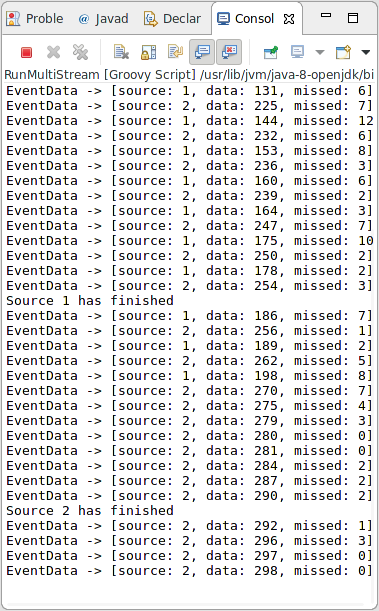
\includegraphics[width=\textwidth/2]{img/screenshots/9-2-1.png}

\textbf{Test 2}

Event sources = 2

EventSource.minTimes = [ 0, 0, 0, 0, 0, 0, 0, 0, 0 ]

EventSource.maxTimes = [ 1, 1, 1, 1, 1, 1, 1, 1, 1 ]

EventProcessing.minTime = 399

EventProcessing.maxTime = 400

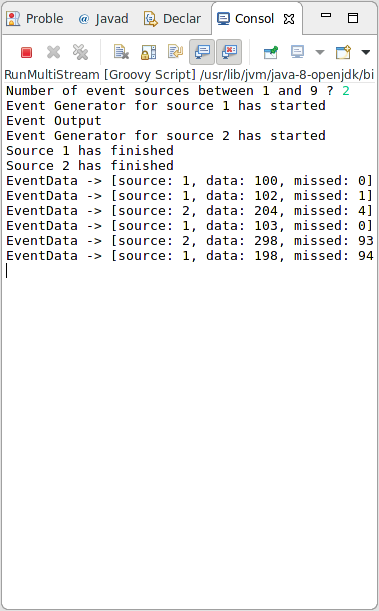
\includegraphics[width=\textwidth/2]{img/screenshots/9-2-2.png}

\textbf{Test 3}

Event sources = 2

EventSource.minTimes = [ 399, 399, 399, 399, 399, 399, 399, 399, 399 ]

EventSource.maxTimes = [ 400, 400, 400, 400, 400, 400, 400, 400, 400 ]

EventProcessing.minTime = 0

EventProcessing.maxTime = 1

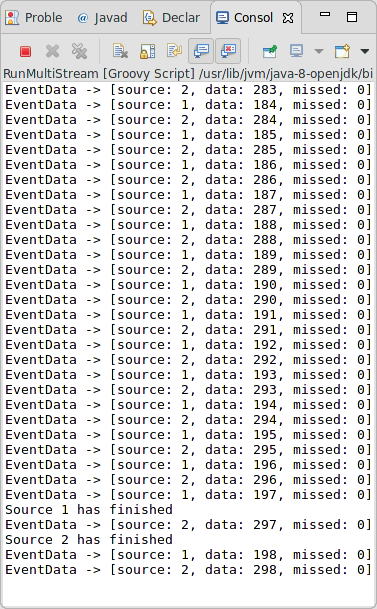
\includegraphics[width=\textwidth/2]{img/screenshots/9-2-3.png}

\textbf{Test 4}

Event sources = 9

EventSource.minTimes = [ 0, 0, 0, 0, 0, 0, 0, 0, 0 ]

EventSource.maxTimes = [ 1, 1, 1, 1, 1, 1, 1, 1, 1 ]

EventProcessing.minTime = 399

EventProcessing.maxTime = 400

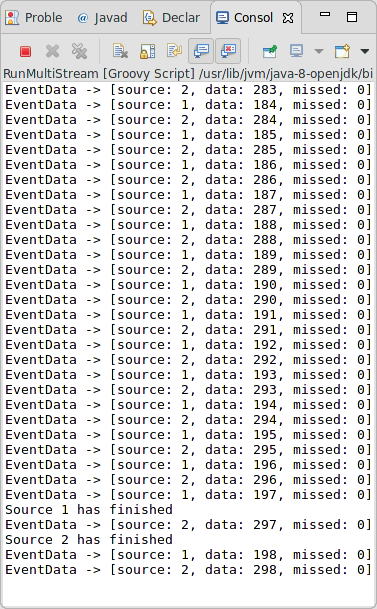
\includegraphics[width=\textwidth/2]{img/screenshots/9-2-3.png}

\textbf{Test 5}

Event sources = 9

EventSource.minTimes = [ 399, 399, 399, 399, 399, 399, 399, 399, 399 ]

EventSource.maxTimes = [ 400, 400, 400, 400, 400, 400, 400, 400, 400 ]

EventProcessing.minTime = 0

EventProcessing.maxTime = 1

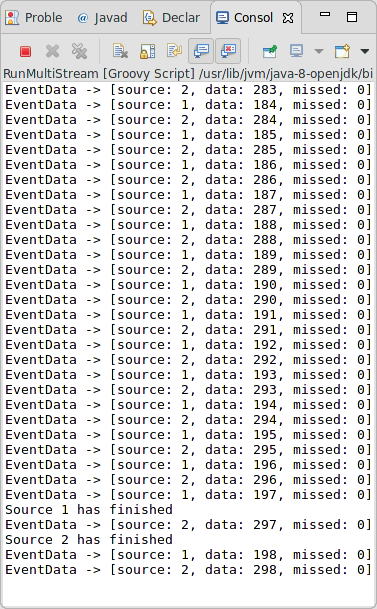
\includegraphics[width=\textwidth/2]{img/screenshots/9-2-3.png}
